\documentclass[aspectratio=169]{beamer}
\usetheme{hogent}
\usecolortheme{hgwhite} % witte achtergrond, zwarte tekst

%% common.tex -- Code die in elk .tex-bestand terug komt

%% Packages

\usepackage[dutch]{babel}
\usepackage{graphicx}
\usepackage{comment,enumerate,hyperref}
\usepackage{amsmath,amsfonts,amssymb}
\usepackage{eurosym}
\usepackage{booktabs}
\usepackage{multicol,multirow}
\usepackage{listings}

\usepackage[outputdir=out]{minted}
%\usepackage{minted}

\usepackage[backend=biber,style=apa]{biblatex}
\DeclareLanguageMapping{dutch}{dutch-apa}

\usepackage{csquotes}

%% Variabelen, elk academiejaar aan te passen
\newcommand{\academicyear}{2023--2024 (revisie: \today)}
\newcommand{\lecturers}{Thomas Aelbrecht \and Thomas Parmentier \and Bert Van Vreckem}
\newcommand{\coursename}{Research Methods (IT)}

%% Macro's en commando's

%% \alertbox: een kader voor tekst die moet opvallen
\newcommand{\alertbox}[2][hgblue]{%
  \setbeamercolor{alertbox}{bg=#1,fg=white}
  \begin{beamercolorbox}[sep=2pt,center]{alertbox}
    \textbf{#2}
  \end{beamercolorbox}
}

\addbibresource{rm4-bibliografie.bib}

%---------- Info over de presentatie ------------------------------------------

\title{Module 4. Een bibliografische databank bijhouden.}
\subtitle{\coursename}
\author{\lecturers}   % Pas waarden aan in common.tex
\date{\academicyear}

\begin{document}

\begin{frame}
  \maketitle
\end{frame}

\begin{frame}
  \frametitle{Inhoud}

  \tableofcontents
\end{frame}

\section{Bronvermeldingen en referentielijst in {\LaTeX}.}

\begin{frame}[plain]
  \frametitle{Opmaken referentielijst.}

  Doel referentielijst = lezers toelaten:

  \begin{itemize}
    \item De gerefereerde bronnen op te zoeken
    \item Waarde bronnen zelf te beoordelen
  \end{itemize}

  {\pause}

  Strikte, vastgelegde vorm:

  \begin{itemize}
    \item Vastgelegde regels, afh.~publicatie (bv. APA, Chicago Manual of Style, IEEE, \ldots)
    \item Vaste volgorde (volgorde in de tekst of alfabetisch)
    \item Lijst met URL's is onvoldoende!
  \end{itemize}

  {\pause}

  \alertbox{Gebruik \textcolor{hgyellow}{referentie-software} om je referentielijst op te maken!}
\end{frame}

\begin{frame}
  \frametitle{Bibliografische databank}

  \begin{itemize}
    \item = Software om bronnen gestructureerd bij te houden
    \item Fulltext + metadata
    \item Genereren correct opgemaakte literatuurlijst
    \item Syn.: reference management software
  \end{itemize}

\end{frame}

\begin{frame}
  \frametitle{Voorbeelden}

  \begin{itemize}
    \item Endnote: commercieel
    \item Mendeley: commercieel, gratis
    \item JabRef: open source
  \end{itemize}

\end{frame}

\begin{frame}[plain]
  \frametitle{JabRef}

  \centering
  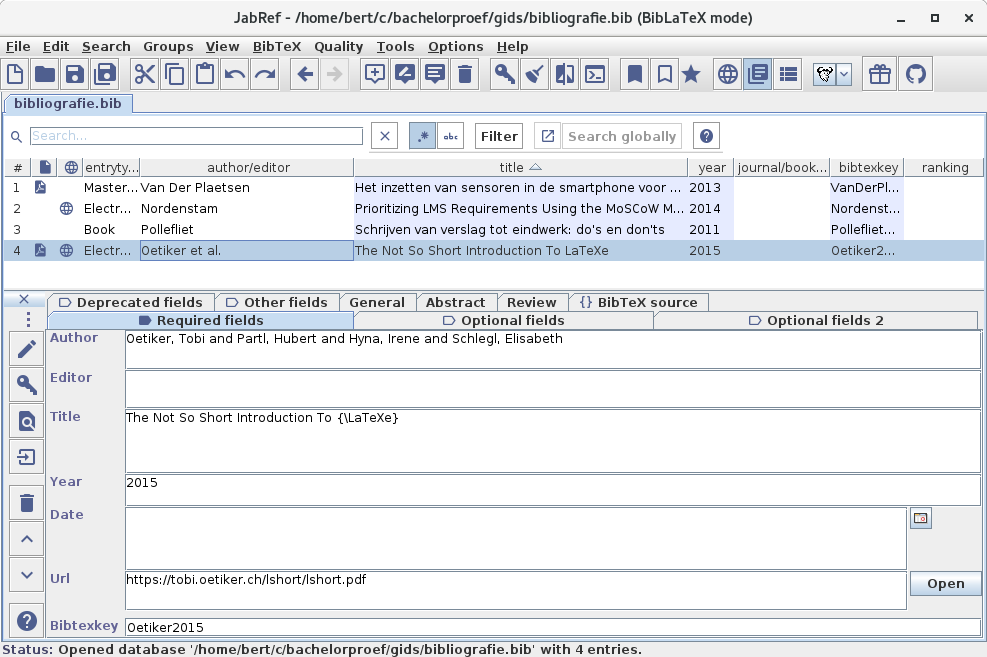
\includegraphics[height=.8\textheight]{4/jabref-screenshot}

\end{frame}

\begin{frame}
  \frametitle{JabRef instellingen}

  \begin{itemize}
    \item Zie \url{https://hogenttin.github.io/latex-hogent-gids/installatie-jabref/}
  \end{itemize}

\end{frame}

\begin{frame}[fragile]
  \frametitle{Bronvermelding en referentielijst in {\LaTeX}.}

  Bib{\LaTeX} en Biber

  \bigskip

  \verb|artikel.tex|: Hoofdtekst\\
  \verb|artikel.bib|: Bibliografische databank (bewerk met bv.~JabRef)

  \bigskip

  Preamble:

  \begin{verbatim}
  \usepackage[backend=biber,style=apa]{biblatex}
  \DeclareLanguageMapping{dutch}{dutch-apa}
  \addbibresource{artikel.bib}
  \end{verbatim}

  \textbf{Opm.}\ Reeds voorzien in het sjabloon!

\end{frame}

\section{Een bibliografische databank aanleggen.}

\begin{frame}
  \frametitle{Bibliografische gegevens in Jabref.}

  Info die \textbf{altijd} ingevuld moet worden:

  \begin{description}
    \item[Author] Persoon/Organisatie opgegeven als auteur
    \item[Title] v/h artikel, boek, \ldots
    \item[Date] (of Year): datum van publicatie (\texttt{jjjj-mm-dd})
    \item[Citationkey] id van deze bron, gebruikt bij refereren (tip: klik op sleutel-icoon)
  \end{description}

  \bigskip

  Kan je één van deze velden niet invullen? Dan is wellicht geen geschikte bron!
\end{frame}

\begin{frame}
  \frametitle{Het auteursveld}

  Gebruik altijd dit formaat:

  \begin{itemize}
    \item Personen: ``Familienaam, Voornaam and Familienaam, Voornaam and Familienaam, Voornaam\ldots''
    \item Organisatie: tussen accolades bv.\ ``\{The Linux Foundation\}''
  \end{itemize}

\end{frame}

\begin{frame}[fragile,plain]
  \frametitle{Bibliografische gegevens in Jabref.}
  \framesubtitle{Extra info voor Article}

  \begin{description}
    \item[Journal] Naam van het tijdschrift
    \item[Volume] Jaargang
    \item[Number] Nummer binnen de jaargang (optioneel)
    \item[Pages] \verb|mmm--nnn|
  \end{description}

  \bigskip

  \textbf{Voorbeeld:}

  \fullcitebib{Anscombe1973}
\end{frame}

\begin{frame}
  \frametitle{Tip: velden automatisch invullen}

  \begin{itemize}
    \item Elsevier, Springer, \ldots\ hebben Bib\LaTeX{} exportfunctie
    \item Plakken in tabblad ``BibTeX source''
  \end{itemize}

  \bigskip

  \centering
  
\includegraphics[height=.6\textheight]{4/elsevier-cite-doi}

\end{frame}

\begin{frame}
  \frametitle{Tip: velden automatisch invullen}

  \begin{itemize}
    \item DOI = Digital Object Identifier
    \item Unieke code voor een publicatie
    \item Jabref: General > DOI > Get Bibtex data from DOI
  \end{itemize}

  \bigskip

  \centering
  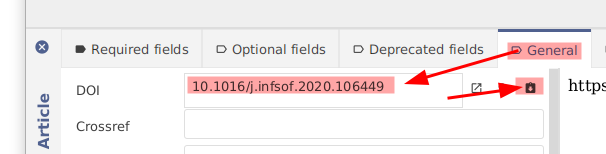
\includegraphics[height=.3\textheight]{4/jabref-doi}

\end{frame}

\begin{frame}[plain]
  \frametitle{Tip: velden automatisch invullen}

  \centering
  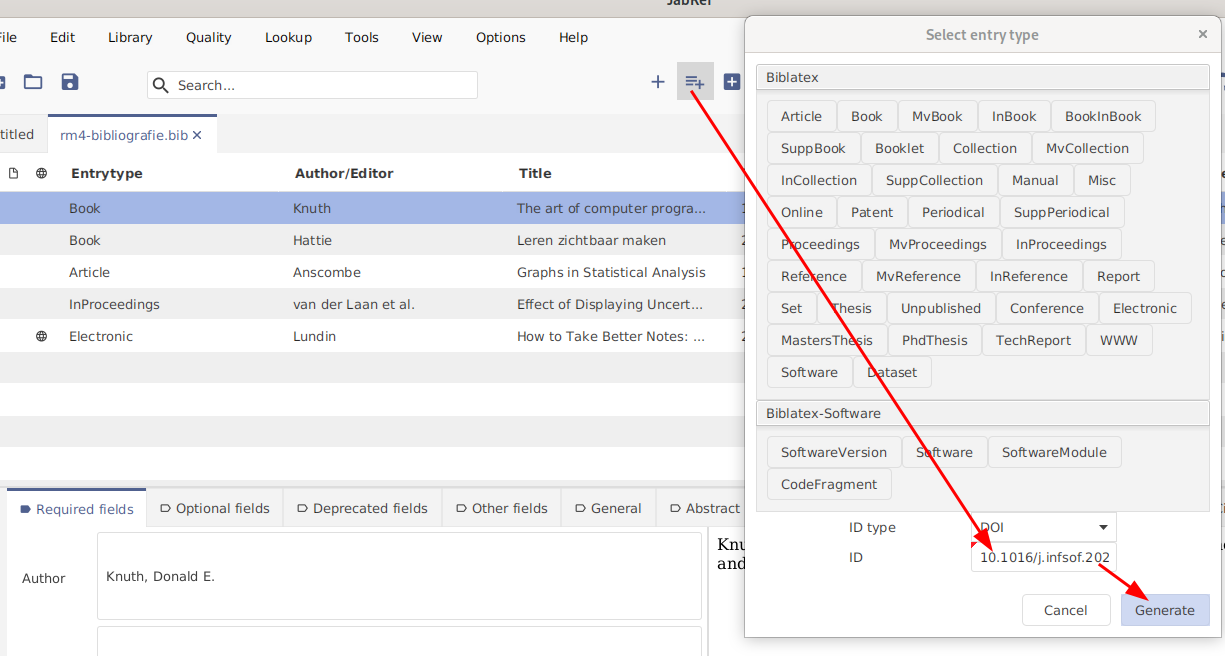
\includegraphics[height=.8\textheight]{4/jabref-new-entry-doi}

\end{frame}

\begin{frame}[plain]
  \frametitle{Bibliografische gegevens in Jabref.}
  \framesubtitle{Extra info voor Online (Electronic, WWW)}

  \begin{description}
    \item[Url] Hyperlink naar de bron
    \item[Urldate] Datum van raadplegen \textbf{VERPLICHT!}
  \end{description}

  \bigskip

  \textbf{Voorbeeld:}

  \bigskip

  \fullcitebib{Lundin2020}

\end{frame}

\begin{frame}[plain]
  \frametitle{Bibliografische gegevens in Jabref.}
  \framesubtitle{Extra info voor InProceedings}

  \begin{description}
    \item[Booktitle] ``Proceedings of the [naam conferentie]''
    \item[Editor] Redacteur(s)
    \item[Pages] paginanummers (optioneel)
  \end{description}

  \medskip

  \textbf{Voorbeeld:}

  \fullcitebib{vanderLaanEtAl2015}
\end{frame}

\begin{frame}[plain]
  \frametitle{Bibliografische gegevens in Jabref.}
  \framesubtitle{Extra info voor Book}

  \begin{description}
    \item[Publisher] Uitgever
    \item[Address] Vestigingsplaats uitgever
  \end{description}

  \medskip

  URL opgeven is ongebruikelijk, tenzij online gepubliceerd!
  
  Webpagina bij uitgever kan, Google books of illegale downloadsite niet!

  \medskip

  \textbf{Voorbeeld:}

  \fullcitebib{Knuth1998}
\end{frame}

%% TODO: report, thesis

\begin{frame}
  \frametitle{Bibliografische gegevens in JabRef.}
  \framesubtitle{Extra info voor Report/Thesis}

  \begin{description}
    \item[Institution] Instelling
    \item[Type] Soort rapport (dropdown in JabRef)
    \item[URL]  en Urldate (indien online gepubliceerd)
  \end{description}

\end{frame}

\begin{frame}[plain]

  \textbf{Voorbeeld bachelorproef:}

  \fullcitebib{VanDerPlaetsen2013}

  \medskip

  \textbf{Voorbeeld onderzoekssrapport:}

  \fullcitebib{DeMarez2022}

\end{frame}

\begin{frame}
  \frametitle{Bibliografische gegevens in JabRef.}

  Vul zoveel mogelijk info in (maakt zoeken eenvoudiger):

  \begin{description}
    \item[DOI] Digital Object Identifier: uniek ID voor artikel, hiermee kan je automatisch alle velden invullen
    \item[URL] ook al is het niet echt een Online bron
    \item[Keywords] Sleutelwoorden
    \item[File] PDF van de publicatie
    \item[Abstract] Samenvatting
    \item[Comments] Je eigen samenvatting/opmerkingen
  \end{description}

\end{frame}

\begin{frame}[fragile]
  \frametitle{URLs opschonen}

  \begin{itemize}
    \item Verwijder overbodige info uit URL
      \begin{itemize}
        \item Referer/tracking info
        \item Highlighting (\verb+https://URL#:~:text=HIGHLIGHT+)
      \end{itemize}
    \item Verwijs naar \textit{de oorspronkelijke} bron
      \begin{itemize}
        \item NIET via tertiaire bronnen (Google Books, Arxiv.org, CiteseerX, \ldots)
      \end{itemize}
  \end{itemize}

\end{frame}

\section{Refereren naar de literatuur.}

\begin{frame}[fragile]
  \frametitle{Refereren in de tekst}

  \begin{itemize}
    \item In de eerste zin waarin je de bron gebruikt
    \item \textcolor{hgorange}{\textbf{Binnen}} de zin
  \end{itemize}

  \bigskip
  Twee vormen:

  \begin{itemize}
    \item Narratief: \verb|\textcite{Knuth1998}| \(\Rightarrow{}\) Knuth (1998)
    \item Tussen haakjes: \verb|\autocite{Knuth1998}| \(\Rightarrow{}\) (Knuth, 1998)
  \end{itemize}

\end{frame}

\begin{frame}[fragile,plain]
  \frametitle{Narratieve referenties}
  \framesubtitle{Gebruik \texttt{\textbackslash{}textcite}}

  \ldots\ als de naam van de auteur onderdeel is van de zin:

  \bigskip

  \small
  \begin{verbatim}
An overview is provided in the survey by~\textcite{RibasEtAl2010}.
For a real-life case-study of applying genetic algorithm ``on top''
of a Mixed Integer Linear Programming model, we refer
to~\textcite{BorodinEtAl2011}.
\end{verbatim}
  \normalsize

  \begin{center}
    $\Downarrow$
  \end{center}

  \begin{quotation}
    An overview is provided in the survey by Ribas et al (2010). For a real-life case-study of applying genetic algorithm ``on top'' of a Mixed Integer Linear Programming model, we refer to Borodin et al (2011).
  \end{quotation}
\end{frame}

\begin{frame}[fragile]
  \frametitle{Referentie tussen haakjes}
  \framesubtitle{Gebruik \texttt{\textbackslash{}autocite}}

  \ldots\ als de naam van de auteur GEEN onderdeel is van de zin:

  \medskip

  \small
  \begin{verbatim}
Reinforcement Learning (RL) is a technique that allows an agent
to learn how to maximize a numerical reward
signal~\autocite{SuttonBarto1998}.
\end{verbatim}
  \normalsize

  \begin{center}
    $\Downarrow$
  \end{center}

  \begin{quotation}
    Reinforcement Learning (RL) is a technique that allows an agent to learn how to maximize a numerical reward signal (Sutton and Barto, 1998).
  \end{quotation}

  \bigskip

  Ook: bij letterlijk citaat, bronvermelding afbeelding

\end{frame}

\begin{frame}[fragile]
  \frametitle{Referentielijst toevoegen.}

  \begin{itemize}
    \item Literatuurlijst invoegen: \verb|\printbibliography|

    \item Compileren (in TexStudio):

          \begin{enumerate}
            \item Build/Compile (F5): bronnen worden nog niet toegevoegd, ``keys'' van bronnen in het vet aangeduid
            \item Bibliography (F8): selecteert de gerefereerde bronnen en maakt ze klaar
            \item Build/Compile (F5): effectief invoegen verwijzingen en literatuurlijst
          \end{enumerate}

    \item In VSCode: gebruik recept ``XeLaTex $\rightarrow$ biber $\rightarrow$ XeLaTeX $\times$ 2''
  \end{itemize}
\end{frame}

\begin{frame}[fragile]
  \frametitle{Controleer het resultaat!}

  \begin{itemize}
    \item Ontbreken er een/meerdere bronnen?
      \begin{itemize}
        \item Enkel bronnen die in de tekst gebruikt worden, verschijnen in de literatuurlijst
        \item Verwijs er naar met \verb|\textcite{}| of \verb|\autocite{}|
        \item \verb|\nocite{*}| toevoegen is niet toegelaten
      \end{itemize}
       
    \item Auteurs correct weergegeven?
    \item Taal- of zetfouten? Bv.\ accentletters, speciale tekens
    \item Alle info om bron terug te vinden aanwezig?
    \item Vermelding ``Verkregen DATUM, van URL'' bij Online bronnen?
    \item \textbf{LET OP!} Speciale tekens (\%, \&, \$, \ldots) zijn ook in .bib verboden, en ook in velden die niet gebruikt worden in de PDF!
    \item \ldots
  \end{itemize}

\end{frame}

\begin{frame}[fragile]
  \frametitle{Tip: bibla}

  \begin{itemize}
    \item \url{https://pypi.org/project/bibla/}
    \item Linter/style checker voor BibLaTeX-bestanden
    \item Controleert op veelgemaakte fouten
    \item Door oud-student HOGENT Tristan Cuvelier
  \end{itemize}

  \begin{verbatim}
    pip install bibla
    bibla lint bibliografie.bib
  \end{verbatim}

\end{frame}

\begin{frame}[plain]
  \frametitle{Vaak voorkomende problemen}
  \framesubtitle{Literatuurlijst}

  \begin{itemize}
    \item Onbruikbare bronnen (bv.\ StackOverflow, Wikipedia, blogs niet van een vakexpert, websites, \ldots)
    \item Foutief type bron (bv. \texttt{Online} in plaats van \texttt{Book} of \texttt{Article}, \ldots)
    \item Incorrecte of ontbrekende info (bv.\ ontbrekende paginanummers, verkeerde volgorde van auteurs, verkeerde auteur \ldots)
    \item COPY/PASTE VAN TITELS IN ALL CAPS. Herschrijf deze!
    \item Niet opgeruimde URLs weergegeven
    \item URL van illegale downloadsite opgegeven
    \item Door ChatGPT gegenereerde bronnen die niet bestaan
    \item \ldots
  \end{itemize}
\end{frame}

\begin{frame}
  \frametitle{Vaak voorkomende problemen}
  \framesubtitle{Verwijzingen}

  \begin{itemize}
    \item Afbeelding zonder bronvermelding (= \textcolor{hgorange}{\textbf{Plagiaat!!}})
    \item Beweringen, definities vaktermen zonder bronvermelding
    \item Verwijzen naar bronnen die bewering in de tekst niet ondersteunen
    \item Verwijzingen buiten de zin
    \item Verwijzingen op einde paragraaf ipv in eerste zin waar bron gebruikt wordt
    \item Te veel tekst gebaseerd op dezelfde bron (max.\ enkele zinnen!)
    \item \ldots
  \end{itemize}

\end{frame}

\begin{frame}[plain]
  \frametitle{Oefening}

  Sla deze bronnen op in JabRef, met alle nodige info en fulltext (waar mogelijk) en/of URL van de online bron:

  \bigskip

  \begin{itemize}
    \item \url{https://www.sciencedirect.com/science/article/abs/pii/S0020025510002756}
    \item \url{https://catalogus.hogent.be/catalog/hog01:000617334}
    \item \url{https://martinfowler.com/articles/microservices.html}
    \item \url{https://www.youtube.com/watch?v=wW9CAH9nSLs&t=13s}
    \item \url{https://link.springer.com/book/10.1007/978-1-4842-6399-0}
    \item \url{https://link.springer.com/chapter/10.1007/978-3-031-27199-1_1}
    \item \url{https://docs.ansible.com/ansible-core/devel/index.html}
  \end{itemize}

\end{frame}

\begin{frame}
  \frametitle{Opdracht}

  \begin{itemize}
    \item Sla alle tijdens literatuurstudie gevonden bronnen op in .bib-bestand
    \item Structureren, bv.\ ahv Mind Map
          \begin{itemize}
            \item Freemind, Gitmind, Xmind, Minder, Vym, \ldots
          \end{itemize}
    \item Verwerk wat je gelezen hebt tot een doorlopende tekst
  \end{itemize}

  \bigskip

  \alertbox{Dit is de belangrijkste fase van de opdracht!}
\end{frame}

\end{document}
